%%
% Please see https://bitbucket.org/rivanvx/beamer/wiki/Home for obtaining beamer.
%%
\documentclass{beamer}

\usepackage{amssymb,amsmath}

%\usepackage{refcheck}

\usepackage{graphicx}
\usepackage{amssymb}
\usepackage{mathrsfs}
\usepackage{amsmath}
\usepackage{latexsym}
\usepackage{amssymb}
\usepackage{enumerate}
\usepackage{color}
%\usepackage{ dsfont }
\usepackage{float}
\usepackage{physics}

%new math symbols taking no arguments
\newcommand\0{\mathbf{0}}
\newcommand\CC{\mathbb{C}}
\newcommand\FF{\mathbb{F}}
\newcommand\NN{\mathbb{N}}
\newcommand\QQ{\mathbb{Q}}
\newcommand\RR{\mathbb{R}}
\newcommand\ZZ{\mathbb{Z}}
\newcommand\bb{\mathbf{b}}
\newcommand\kk{\Bbbk}
\newcommand\mm{\mathfrak{m}}
\newcommand\pp{\mathfrak{p}}
\newcommand\xx{\mathbf{x}}
\newcommand\yy{\mathbf{y}}
\newcommand\GL{\mathit{GL}}
\newcommand\into{\hookrightarrow}
\newcommand\nsub{\trianglelefteq}
\newcommand\onto{\twoheadrightarrow}
\newcommand\minus{\smallsetminus}
\newcommand\goesto{\rightsquigarrow}
\newcommand\nsubneq{\vartriangleleft}

%redefined math symbols taking no arguments
\newcommand\<{\langle}
\renewcommand\>{\rangle}
\renewcommand\iff{\Leftrightarrow}
\renewcommand\phi{\varphi}
\renewcommand\implies{\Rightarrow}

%new math symbols taking arguments
\newcommand\ol[1]{{\overline{#1}}}

%redefined math symbols taking arguments
\renewcommand\mod[1]{\ (\mathrm{mod}\ #1)}

%roman font math operators
\DeclareMathOperator\aut{Aut}

%for easy 2 x 2 matrices
\newcommand\twobytwo[1]{\left[\begin{array}{@{}cc@{}}#1\end{array}\right]}

%for easy column vectors of size 2
\newcommand\tworow[1]{\left[\begin{array}{@{}c@{}}#1\end{array}\right]}

%\newtheorem{theorem}{Theorem}[section]
%\newtheorem{corollary}{Corollary}[theorem]
\newtheorem{proposition}{Proposition}[theorem]
\newtheorem{algorithm}{Algorithm}[theorem]
%\newtheorem{lemma}[theorem]{Lemma}
%\newtheorem{exercise}[theorem]{Exercise}
%\newtheorem{definition}[theorem]{Definition}

\title{Quantum-inspired $\ell^2$ sampling}
\subtitle{and applications to machine learning}
\author[Sbahi] % (optional, for multiple authors)
{Faris Sbahi}
\date{3/5/19}
\subject{Physics}

\begin{document}
\maketitle

\AtBeginSection[]
{
  \begin{frame}<beamer>
    \tableofcontents[currentsection]
  \end{frame}
}

\section{Machine Learning}

\begin{frame}
    \frametitle{Machine Learning}
    \framesubtitle{Introduction}
    \begin{itemize}
    \item Machine learning is a broad term for algorithms which are capable of finding patterns in data.
    \item Fundamental goal: capture these patterns in a "model" that \textit{generalizes} to unseen data.
    \item These algorithms have two components:
    \begin{enumerate}
    \item A learning element. Updates the model depending on its performance on the considered dataset.
    \item A performance element. Provides the measure of performance.
    \end{enumerate}
	\item Bottom line: "machine learning" is a somewhat hollow term. Many ML algorithms are in fact familiar linear algebraic techniques.
    \end{itemize}
    \end{frame}

% Goal is simply to show why these linear algebraic techniques can be regarded as machine learning algorithms
  \begin{frame}
  	\frametitle{PCA}
    \framesubtitle{Motivation: Singular value transformation}
    \begin{itemize}
    \item "Training" dataset $\mathcal{T}$ consists of the accessible samples of data. $\mathcal{T}$ is drawn from a subset of $\Omega \subset \RR^d$ where each component represents a "feature". 
    \item Samples from $\Omega$ are assumed to be drawn according to some distribution $\mathcal{D}$. 
    \item Example: data is collected on the heights and lengths of cherry blossom petals. 
    \begin{figure}
   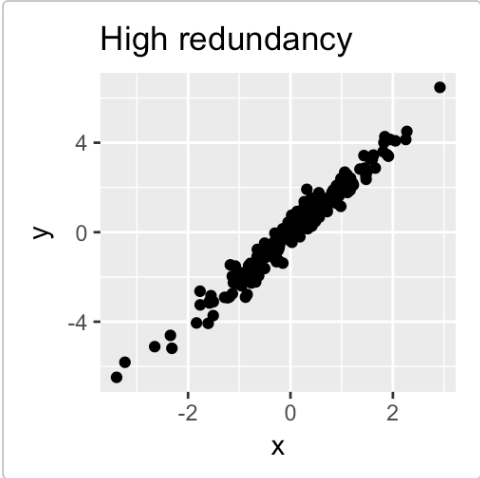
\includegraphics[width= 0.3\linewidth]{pca_high_redundancy.png}
   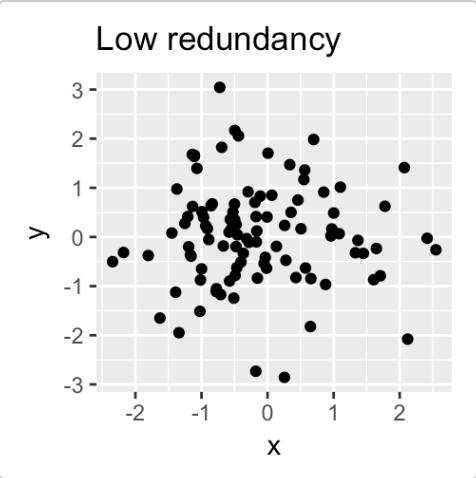
\includegraphics[width= 0.3\linewidth]{pca_low_redundancy}	
\end{figure}
\item How and why may it make sense to reduce the dimensionality of the feature space?
\end{itemize}
\end{frame}

\begin{frame}
\frametitle{Moore-Penrose Pseudoinverse}
    \framesubtitle{Motivation: Singular value transformation}
    \begin{itemize}
    \item Let $A \in \CC^{m \times n}$ and $b \in \CC^m$ unit vector.
    \item We wish to find the $x_{LS}$ which satisfies $x_{LS} = \arg\min_{x} \| Ax - b \|_2$
    \item Notation: $x_{LS} = A^+ b$
    \item Common strategy uses SVD: write $A = UDV^\dag$ and then $A^+ = VD^+U^\dag$ where $D^+$ simply inverts the non-zero diagonal entries.
    \end{itemize}
	\begin{figure}
   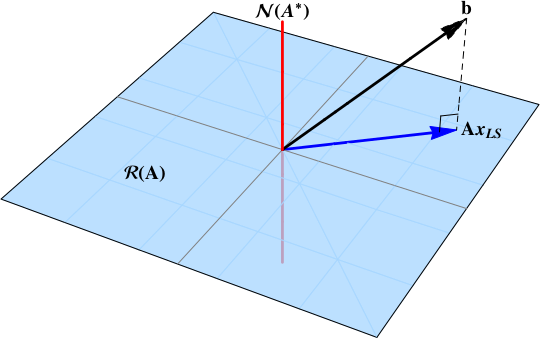
\includegraphics[width= 0.5\linewidth]{least-squares.png}	
\end{figure}
\end{frame}

\section{Quantum Machine Learning}

\begin{frame}
\frametitle{Moore-Penrose Pseuodinverse}
\framesubtitle{Harrow, Hassidim, Lloyd (orig.) Wiebe, Braun} 
\begin{itemize}
    \item HHL algorithm: application of phase estimation and Hamiltonian simulation to solve linear system.
    \item We can use HHL as a subroutine to compute $A^+ \ket{b} = \ket{x}$ in ($\ket{x}$ is the least-square solution).
    \item Note that $\ket{x}$ is a quantum state. Hence, we may efficiently measure an expectation value $x^T M x$ where $M$ is some p.s.d operator.
    \item Runtime bound $\tilde{O}(log(N)(s^3\kappa^6)/ \epsilon)$ time (query complexity)
    \item Assumption: $A$ is sparse with low condition number $\kappa$. Hamiltonian simulation is efficient when $\hat{H}$ is sparse. No low-rank assumptions are necessary.
    \item "Key" assumption: the quantum state $\ket{b}$ can be prepared efficiently.	
    

\end{itemize}
\end{frame}

\begin{frame}
\frametitle{Read the Fine Print}	
\begin{itemize}
\item In general QML algorithms convert quantum input states to the desired quantum output state. 
\item In practice, data is initially stored classically and the algorithm's output must be accessed classically as well.
\item This poses two problems if seek to use these algorithms: the "state preparation" and "readout" problems.
\item Even if we ignore the readout problem, can we at least find a state preparation routine that maintains a speedup for the discussed quantum algorithms? Open question!
\item See "Quantum Machine Learning Algorithms: Read the Fine Print" by Aaronson
\end{itemize}
\end{frame}

\section{Classical $\ell^2$ sampling}

\begin{frame}
\frametitle{In search of a "fair" comparison}	

\begin{itemize}
\item How can we compare the speed of quantum algorithms with quantum input and quantum output to classical algorithms with classical input and classical output? 
\item Quantum machine learning algorithms can be exponentially faster than the best standard classical algorithms for similar tasks, but this comparison is unfair because the quantum algorithms get outside help through input state preparation. 
\item We want a classical model that helps its algorithms stand a chance against quantum algorithms, while still ensuring that they can be run in nearly all circumstances one would run the quantum algorithm. 
\item Solution (Tang): compare quantum algorithms with quantum state preparation to classical algorithms with sample and query access to input.	
\end{itemize}
\end{frame}

% how to compare? query complexity
% what kind of data structure allows for l-s sampling

\begin{frame}
\frametitle{Classical $\ell^2$ Sampling Model}
\begin{definition}
We have "query access" to $x \in \CC^n$ if, given $i \in [n]$, we can efficiently compute $x_i$. We say that $x \in \mathcal{Q}$.
\end{definition}
\begin{definition} Definition. We have sample and query access to $x \in \CC^n$ if we have query access to $x$; can produce independent random samples $i \in [n]$ where we sample $i$ with probability $|x_i|^2/\|x\|^2∣x $ and can query for $\|x\|$. We say that $x \in \mathcal{SQ}$. 
\end{definition}
\begin{definition} Definition. For $A \in \CC^{m\times n}$, $A \in \mathcal{SQ}$ (abuse) iff $A_i \in \mathcal{SQ}$ for $A_i$ the rows of $A$, along with $\tilde{A} \in \mathcal{SQ}$ for $\tilde{A}$ the vector of row norms (so $\tilde{A}_i = \|A_i\|$).
\end{definition}
\end{frame}

\begin{frame}
\frametitle{"Dequantization" (Tang)}
\begin{definition}
 Let $\mathcal{A}$ be a quantum algorithm with input $\ket{\phi_1},\ldots,\ket{\phi_C}$ and output either a state $\ket{\psi}$ or a value $\lambda$. We say we dequantize $\mathcal{A}$ if we describe a classical algorithm that, given $\phi_1,\ldots,\phi_C \in \mathcal{SQ}$, can evaluate queries to $\psi \in \mathcal{SQ}$ or output $\lambda$, with similar guarantees to $\mathcal{A}$ and query complexity $\text{poly}(C)$.	
\end{definition}
\end{frame}

\begin{frame}
\frametitle{Dequantization Toolbox}
\framesubtitle{Method 1: Inner product estimation (Tang, 2018)}
\begin{itemize}
	\item For $x, y \in \CC^n$, if we are given that $x \in \mathcal{SQ}$ and $y \in \mathcal{Q}$, then we can estimate $\< x, y\>$ with probability $\geq 1 - \delta$ and error $\epsilon \|x\|\|y\|$ 
	\item Quantum analogue: SWAP test
\end{itemize}
\begin{figure}
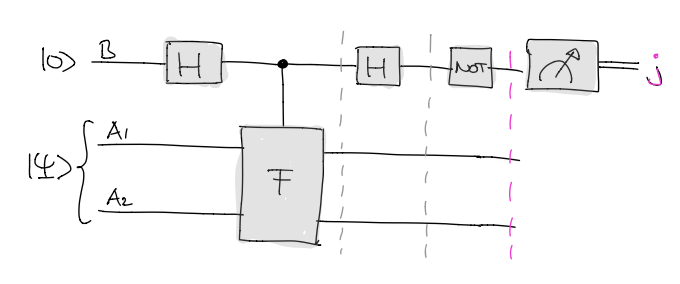
\includegraphics[width= 0.5\linewidth]{swap_test.png}	
\end{figure}
\end{frame}

\begin{frame}
\frametitle{Dequantization Toolbox}
\framesubtitle{Method 1: Inner product estimation (Tang, 2018)}
\begin{fact} For $\{X_{i,j}\}$ i.i.d random variables with mean $\mu$ and variance $\sigma^2$, let 

$$Y := \underset{j \in [6\log 1/\delta]}{\operatorname{median}}\;\underset{i \in [6/\epsilon^2]}{\operatorname{mean}}\;X_{i,j}$$ 

Then $\vert Y - \mu\vert \leq \epsilon\sigma$ with probability $\geq 1-\delta$, using only $O(\frac{1}{\epsilon^2}\log\frac{1}{\delta})$ copies of $X$.
\end{fact}
\begin{proof} (sketch) The proof follows from two facts: 

\begin{itemize}
\item first, the median of $C_1,\ldots,C_n$ is at least $\lambda$ precisely when at least half of the $C_i$ are at least $\lambda$; 
\item second, Chebyshev's inequality (applied to the mean).
\end{itemize}
\end{proof}
\end{frame}

\begin{frame}
\frametitle{Dequantization Toolbox}
\framesubtitle{Method 1: Inner product estimation (Tang, 2018)}
\begin{corollary} For $x,y \in\CC^n$, given $\mathcal{SQ}(x)$ and $\mathcal{Q}(y)$, we can estimate $\langle x,y\rangle$ to $\epsilon\|x\|\|y\|$ error with probability $\geq 1-\delta$ with query complexity $O(\frac{1}{\epsilon^2}\log\frac{1}{\delta})$
\end{corollary}

\begin{proof}Sample $s$ from $v$ and let $Z = x_s v_s\frac{\|v\|^2}{|v_s|^2}$. Apply the Fact with $X_{i,j}$ being independent copies of $Z$.
\end{proof}	
\end{frame}

\begin{frame}
\frametitle{Dequantization Toolbox}
\framesubtitle{Method 2: Thin Matrix-Vector (Tang, 2018)}
\begin{itemize}
	\item For $V \in \CC^{n\times k}, w \in \CC^k$, given $V^\dagger \in \mathcal{SQ}$ (i.e. column-wise of $V$) and $w \in \mathcal{Q}$, we can simulate $Vw \in \mathcal{SQ}$ with $\text{poly}(k)$ queries
	\item Quantum analogue: SWAP test
\end{itemize}
\begin{figure}
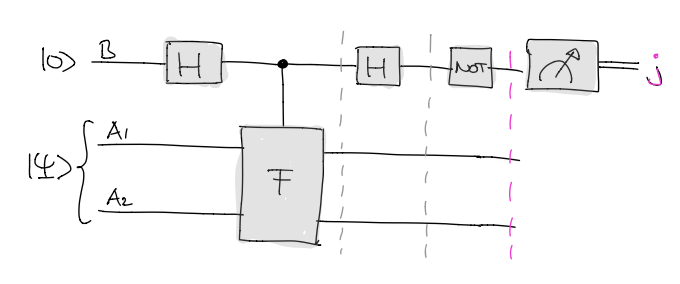
\includegraphics[width= 0.5\linewidth]{swap_test.png}	
\end{figure}
\end{frame}

\begin{frame}
\frametitle{Dequantization Toolbox}
\framesubtitle{Method 2: Thin Matrix-Vector (Tang, 2018)}
\begin{definition}
Rejection sampling
\end{definition}
\begin{algorithm}
Input: Samples from distribution $P$

Output: Samples from distribution $Q$
\begin{itemize}
\item Sample $s$ from $P$
\item Compute $r_s = \frac{1}{M}\frac{Q(s)}{P(s)}$ 
\item Output $s$ with probability $r_s$ and restart otherwise
\end{itemize}
\end{algorithm}

\begin{fact}
Fact. If $r_i \leq 1, \forall i$, then the above procedure is well-defined and outputs a sample from $Q$ in $M$ iterations in expectation.	
\end{fact}


\end{frame}

\begin{frame}
\frametitle{Dequantization Toolbox}
\framesubtitle{Method 2: Thin Matrix-Vector (Tang, 2018)}
\begin{proposition}
	 For $V \in \RR^{n\times k}$ and $w \in \RR^k$, given $V \in \mathcal{SQ}$ and $w \in \mathcal{Q}$, we can simulate $Vw \in \mathcal{SQ}$ with expected query complexity $O(k^2C(V,w))$, where

$$C(V,w) := \frac{\sum_{i=1}^k\|w_iV^{(i)}\|^2}{\|Vw\|^2}$$

We can compute entries $(Vw)_i$ with $O(k)$ queries.

We can sample using rejection sampling:

\begin{itemize}
\item $P$ is the distribution formed by sampling from $V^{(j)}$ with probability proportional to $\|w_jV^{(j)}\|^2$
  
\item $Q$ is the target $Vw$.
\end{itemize}

$$r_i = \frac{(Vw)_i^2}{k \sum_{j=1}^k (w_jV_{ij})^2} = \frac{Q(i)}{kC(V,w)P(i)}$$
\end{proposition}
\end{frame}

\begin{frame}
\frametitle{Dequantization Toolbox}
\framesubtitle{Method 2: Thin Matrix-Vector (Tang, 2018)}
\begin{itemize}
\item Notice that we can compute these $r_i$'s (in fact, despite that we cannot compute probabilities from the target distribution), and that the rejection sampling guarantee is satisfied (via Cauchy-Schwarz).

\item The probability of success is $\frac{\|Vw\|^2}{k\sum_{i=1}^k\|w_iV^{(i)}\|^2}$. Thus, to estimate the norm of $Vw$, it suffices to estimate the probability of success of this rejection sampling process.

\item Through a Chernoff bound, we see that the average of $O(kC(V,w)(\frac{1}{\epsilon^2}\log\frac{1}{\delta}))$ "coin flips" is in $[(1-\epsilon)\|Vw\|,(1+\epsilon)\|Vw\|]$ with probability $\geq 1-\delta$, where each coin flip costs $k$ queries and samples.	
\end{itemize}
\end{frame}


\begin{frame}
\frametitle{Dequantization Toolbox}
\framesubtitle{Method 3: Low-Rank Approximation (Frieze, Kannan, Vempala, 1998)}
\begin{itemize}
\item For $A \in \CC^{m\times n}$, given $A \in \mathcal{SQ}$ and some threshold $k$, we can output a description of a low-rank approximation of $A$ with $\text{poly}(k)$ queries.
\item Specifically, our output is $\mathcal{SQ}(S,\hat{U})$ for $S \in \CC^{\ell \times n}$, $\hat{U} \in \CC^{\ell \times k}$ ($\ell = \text{poly}(k,\frac{1}{\epsilon}$), and this implicitly describes the low-rank approximation to $A$, $D := A(S^\dagger\hat{U})(S^\dagger\hat{U})^\dag$ (notice rank $D \leq k$).

\item This matrix satisfies the following low-rank guarantee with probability $\geq 1-\delta$: for $\sigma := \sqrt{2/k}\|A\|_F$, and $A_{\sigma} := \sum_{\sigma_i \geq \sigma} \sigma_iu_iv_i^\dag$ (using SVD), 
$$\|A - D\|_F^2 \leq \|A - A_\sigma\|_F^2 + \epsilon^2\|A\|_F^2$$
\item This guarantee is non-standard: instead of $A_k$, we use $A_\sigma$. This makes our promise weaker, since it is useless if $A$ has no large singular values.
\item Quantum analogue: phase estimation
\end{itemize}
\end{frame}

\begin{frame}
\frametitle{Moore-Penrose Pseudoinverse (low-rank)} 	
\framesubtitle{Application}

\begin{problem} For a low-rank matrix $A \in \RR^{m\times n}$
  and a vector $x \in \RR^n$, given $x, A \in \mathcal{SQ}$, (approximately) respond to requests for $A^+x \in \mathcal{SQ}$, where $A^+$ is the pseudoinverse of $A$. 
\end{problem}
\begin{algorithm}   	
\begin{itemize}
\item Use the low-rank approximation protocol (3) to get $\mathcal{SQ}(S,\hat{U})$.

\item From applying the matrix-vector protocol (2), we have $\mathcal{SQ}(\hat{V})$, where $\hat{V} := S^T\hat{U}$; we can show that the columns of $\hat{V}$ behave like the right singular vectors of $A$. 

\item Further, (3) also outputs their approximate singular values $\hat{\sigma}_i$
 
\item Hence, we can approximate the vector we wish to sample:

$$A^+x = (A^TA)^+A^Tx \approx \sum_{i=1}^k \frac{1}{\hat{\sigma}_i^2}\hat{v}_i\hat{v}_i^T A^Tx$$
\end{itemize}
\end{algorithm}
\end{frame}

\begin{frame}
\frametitle{Moore-Penrose Pseudoinverse (low-rank) cont.} 	
\framesubtitle{Application}
\begin{itemize}
\item We approximate $\hat{v}_i^TA^Tx$ to additive error for all by noticing that $\hat{v}_i^TA^Tx = \Tr(A^Tx\hat{v}_i^T)$ is an inner product of the order two tensors $A^TA$ and $x\hat{v}_i^Tx$. 
\item Thus, we can apply (1), since being given $\mathcal{SQ}(A)$ implies $\mathcal{SQ}(A^T)$ for $A^TA$ viewed as a long vector. 
\item Finally, using (2), sample from the linear combination using these estimates and $\hat{\sigma}_i$.	
\end{itemize}
\end{frame}

\section{Remarks}

\begin{frame}
\frametitle{Thoughts}	

\begin{itemize}
\item Conjecture: For machine learning problems, SQ assumptions are more reasonable than state preparation assumptions.
\item We discussed pseuo-inverse which inverts singular values, but in principle we could have applied any function to the singular values
\item Gilyen et. al (2018) show that many quantum machine learning algorithms indeed apply polynomial functions to singular values
\item Our discussion suggests that exponential quantum speedups are tightly related to problems where high-rank matrices play a crucial role (e.g. Hamiltonian simulation of QFT)
\end{itemize}
\end{frame}

% mention qram?

 \end{document}
  
